\chapter{External specification}
\section{Software}
\subsection{Operating system}
Project was developed and tested on Linux operating system.
Installation instructions for the tools used in this thesis are provided for computers with Linux operating system.

\subsection{Programming language}
The code was implemented using Python programming language version 3.12.
To manage project dependencies and environment, virtual environment was used.
For installation of required libraries, built-in Package Installer for Python (pip) was used in version 25.2, that allows to install additional libraries from Python Package Index (PyPI).

\subsection{IDE}
Whole code was written using Visual Studio Code (VS Code) version 1.81.1. While VS Code in itself do not provide full IDE capabilities, it can be extended using various extensions.
For this project, the following extensions were used:
\begin{itemize}
    \item Python extension by Microsoft
    \item Pylez
    \item Jupyter
\end{itemize}

\subsection{Drivers}
To utilize GPU acceleration for model training, NVIDIA GPU drivers in version 580.95.05 were installed as well as CUDA Package in version 13.1.1-1.
These are required to use tensorcores on NVIDIA GPUs for faster computation.

\section{Libraries}
\subsection{Machine learning frameworks}
As the main framework for building and training the models, TensorFlow in version 2.20.0 was used.
It is a Python library for machine learning and artificial intelligence.
It provides a comprehensive ecosystem of tools, libraries, and community resources that lets researchers push the state-of-the-art in ML, and developers easily build and deploy ML-powered applications.
In this thesis, TensorFlow was used mainly for:
\begin{itemize}
    \item Multidimensional arrays
    \item Distributed processing
    \item Model construction and training
\end{itemize}

\paragraph{Other libraries}
\begin{itemize}
    \item {\bf Keras} (version 3.12.0) is a high-level API of TensorFlow that provides an easy-to-use interface for machine learning problems.
          It covers the workflow from data processing to model deployment. \\
          Main advantages of Keras are:
          \begin{itemize}
              \item Simple interface
              \item Clear error messages
              \item Automated multiprocessing
              \item Highly integrated GPU acceleration
          \end{itemize}
    \item {\bf NumPy} (version 2.3.5) is a fundamental mathematical and vector operation library for Python.
          It provides many mathematical functions and data structures useful for performing mathematical operations.
          In this thesis, it was mainly used due to the format of the HSIs and for efficient array manipulations.
    \item {\bf Pandas} (version 2.3.3) is a data analysis and manipulation library.
          It was used for loading and processing CSV files containing dataset splits.
    \item {\bf Matplotlib} (version 3.10.8) is a plotting library used for creating visualizations of results and training progress.
    \item {\bf TensorBoard} (version 2.20.0) is a visualization toolkit for TensorFlow that provides tools for tracking metrics during training.
    \item {\bf Pillow} (version 12.0.0) is an imaging library used for image processing operations.
    \item {\bf scikit-learn} provides the PCA and IncrementalPCA implementations used for the Karhunen-Lo\`eve Transform (KLT).
    \item {\bf pytz} is used for timezone handling when generating timestamps for experiment logs and model checkpoints.
    \item {\bf os} provides bindings for the operating system.
          It is a built-in library in Python.
          It was used mainly for working with the filesystem.
\end{itemize}

\section{Hardware}
The training process was performed on NVIDIA graphics cards due to their CUDA and tensor core capabilities, due to this 2 NVIDIA GPUs were used.
The first one was NVIDIA GeForce RTX 4080 with 16 GB of VRAM.
The second one was NVIDIA GeForce RTX 2080 Ti with 11 GB of VRAM.
Both of the GPUs support CUDA 13.1, and they are equipped with Tensor Cores, which significantly improve machine learning performance.
Some parts of the network training and testing were performed on the CPU when GPU memory was insufficient.
One of the CPUs used was an AMD Ryzen 7 7700X with 8 cores equipped with 32 GB of RAM.
The other one was a dual-socket Intel Xeon E5-2667 v4 equipped with 512 GB of RAM.

\section{Environment setup}
\subsection{Installation}
The project source code can be found in the repository: \url{https://github.com/PiHalves/HSI-Compression}.
To run the project, Python 3.12 is required.
The first step is to create a virtual environment to isolate the project dependencies from the system ones.
The next step is to install the required libraries.
The required libraries are listed in the \mintinline{bash}|requirements.txt| file in the main repository directory.
Both of these steps can be done using the following command in the terminal provided in Figure \ref{fig:venv_creation}.
\begin{figure}[h]
    \centering
    \begin{minted}[linenos,frame=lines]{bash}
Python3.12 -m venv .env
source .env/bin/activate
pip install -r requirements.txt
\end{minted}
    \caption{Creating virtual environment and installing required libraries.}
    \label{fig:venv_creation}
\end{figure}
The complete list of dependencies is specified in the \mintinline{bash}|requirements.txt| file and includes all necessary packages for TensorFlow operations, data processing, and visualization.
Key version requirements include:\par
\begin{itemize}
    \item[Python] $\geq$ 3.12
    \item[TensorFlow] $\geq$ 2.20.0
    \item[Keras] $\geq$ 3.12.0
    \item[NumPy] $\geq$ 2.3.5
    \item[CUDA] $\geq$ 13.1 (for GPU acceleration)
\end{itemize}
\par
\subsection{Dataset}
The dataset used in this project can be downloaded from the following link: \url{https://datadryad.org/dataset/doi:10.5061/dryad.fttdz08zh}
The downloaded dataset will need to be unpacked.
To do that, use this command in the terminal:
\begin{figure}[htbp]
    \centering
    \begin{minted}[linenos,frame=lines]{bash}
    tar -xzf hyspecnet-11k-*.tar.gz
    \end{minted}
    \caption{Unpacking the dataset.}
    \label{fig:unpacking_dataset}
\end{figure}
\par
After unpacking, it is necessary to preprocess the data using the script provided in this repository: \url{https://git.tu-berlin.de/rsim/hyspecnet-tools}.
To do that, download the repository, open the file \mintinline{bash}|tif_to_npy.ipynb| and set variable \mintinline{python}|in_directory| to the path of the unpacked dataset in the second cell of the file.
Run all the cells in the notebook to preprocess the data.
After preprocessing, the folder structure should look like in Figure \ref{fig:preprocessed_data}.

\begin{figure}[htbp]
    \centering
    \begin{forest}
        for tree={
        folder,
        grow'=0,
        fit=band
        }
        [hyspecnet-11k
        [patches
            [tile\_001
                [tile\_001-patch\_01
                    [tile\_001-patch\_01-DATA.npy]
                    [tile\_001-patch\_01-QL\_PIXELMASK.TIF]
                    [\dots]
                ]
                [tile\_001-patch\_02
                    [tile\_001-patch\_02-DATA.npy]
                    [tile\_001-patch\_02-QL\_PIXELMASK.TIF]
                    [\dots]
                ]
                [\dots]
            ]
            [tile\_002
                [tile\_002-patch\_01
                    [tile\_002-patch\_01-DATA.npy]
                    [tile\_002-patch\_01-QL\_PIXELMASK.TIF]
                    [\dots]
                ]
                [\dots]
            ]
            [\dots]
        ]
        [splits
            [easy
                    [train.csv]
                    [val.csv]
                    [test.csv]
            ]
            [hard
                    [train.csv]
                    [val.csv]
                    [test.csv]
            ]
        ]
        ]
    \end{forest}
    \caption{Ready to use dataset structure.}
    \label{fig:preprocessed_data}
\end{figure}

{\bf Best Models } \newline
In the course of the thesis, several models were trained.
The best weights of these models are provided in the directory structure shown in Figure \ref{fig:directory_tree}.
This folder structure is placed in the main repository of the project.

\begin{figure}[tbp]
    \centering
    \begin{forest}
        for tree={
        folder,
        grow'=0,
        fit=band,
        }
        [results
            [lossy
                    [case2d1d.keras]
                    [case3d.keras]
                    [GNN.weights.h5]
            ]
            [lossless
                    [lineRWKV.weights.h5]
            ]
        ]
    \end{forest}
    \caption{Directory tree structure.}
    \label{fig:directory_tree}
\end{figure}

\chapter{Internal specification}

\section{File structure}
The project is organized into several directories and files, each serving a specific purpose.
The repository is structured to clearly separate lossless and lossy compression pipelines, isolate non-learned signal processing components (such as KLT), and decouple training logic from model definitions.
This separation allows independent development and testing of each component while maintaining clear interfaces between them.
The structure is shown in Figure \ref{fig:repo_structure}:\par

\begin{figure}[h]
    \centering
    \begin{forest}
        for tree={
        folder,
        grow'=0,
        fit=band,
        }
        [Repository
            [Code
                    [lossless]
                    [lossy]
                    [segmentation]
                    [TFDataloader]
                    [metrics]
                    [nonML]
                    [main.py]
            ]
            [Latex
                    [Thesis files]
            ]
            [results]
            [requirements.txt]
        ]
    \end{forest}
    \caption{Main project files and directories.}
    \label{fig:repo_structure}
\end{figure}

Description of the elements in the repository shown in Figure \ref{fig:repo_structure}:
\begin{itemize}
    \item {Code/lossless}: Contains the implementation of the LineRWKV model for lossless compression.
    \item {Code/lossy}: Contains the implementation of the lossy compression models (RCGDNAE, RCAE3D, RCAE2D1D).
    \item {Code/segmentation}: Contains the implementation of segmentation models for hyperspectral data classification (small\_segmenter).
    \item {Code/TFDataloader}: Contains the data loader implementation for loading and preprocessing the hyperspectral image dataset.
    \item {Code/metrics}: Contains the implementation of various evaluation metrics used to assess model performance.
    \item {Code/nonML}: Contains the KLT implementation needed for the RCGDNAE model.
    \item {Code/main.py}: The main script to run training and evaluation of the models.
    \item {Latex}: Contains all the files related to the thesis document.
    \item {results}: Contains the best model weights and results from training.
    \item {requirements.txt}: Lists all the Python dependencies required to run the project.
\end{itemize}

\section{Model overview}

Table \ref{tab:model_comparison} summarizes the key characteristics of each implemented model.

\begin{table}[H]
    \centering
    \caption{Comparison of implemented compression models.}
    \label{tab:model_comparison}
    \begin{tabular}{l c c c}
        \hline
        \textbf{Model} & \textbf{Type} & \textbf{Convolution} & \textbf{Key Feature}    \\
        \hline
        LineRWKV       & Lossless      & ---                  & Autoregressive          \\
        RCGDNAE        & Lossy         & 2D + KLT             & Rate--distortion        \\
        RCAE (3D)      & Lossy         & 3D                   & Joint spatial--spectral \\
        CAE2D1D        & Lossy         & 2D + 1D              & Separated processing    \\
        Small Seg      & Segmentation  & 3D + 2D              & Spectral pooling        \\
        \hline
    \end{tabular}
\end{table}


\section{Classes and functions}
\subsection{LineRWKV model}
The lineRWKV model is implemented in the file \mintinline{Python}|Code/lossless/lineRWKV.py| with a trainer class defined in \mintinline{Python}|Code/lossless/lineRWKV_trainer.py|.
There are three classes in the \mintinline{Python}|lineRWKV.py| file: LineRWKVBlock, LineRWKVPredictor, and LineRWKVLosslessCodec.
All of these classes describe the basic building blocks and functionality of the LineRWKV model.
\subsubsection{LineRWKVBlock}
The LineRWKVBlock class implements a single block of the LineRWKV model, inheriting from \mintinline{Python}|tf.keras.layers.Layer|.
This block encapsulates the core RWKV attention mechanism adapted for line-based processing of hyperspectral data, managing the recurrent state updates and attention computations within a single processing unit.
\subsubsection{LineRWKVPredictor}
The LineRWKVPredictor class encapsulates the autoregressive prediction mechanism required for lossless coding of hyperspectral images, inheriting from \mintinline{Python}|tf.keras.Model|.
The predictor processes data line-by-line to maintain causality during encoding and decoding---each line prediction depends only on previously processed lines.
Preprocessing is integrated within the model to ensure consistent data transformation across training and inference.
The \mintinline{Python}|predict_line_by_line| method provides explicit causal prediction, while \mintinline{Python}|compute_residuals| separates residual computation for downstream entropy coding.
This design allows the same model to be used for both training (batch processing) and inference (sequential line processing).
\subsubsection{LineRWKVLosslessCodec}
The LineRWKVLosslessCodec class provides a complete encode/decode interface for lossless compression, wrapping the LineRWKVPredictor.
This separation of concerns allows the predictor to focus on prediction quality while the codec handles the compression workflow---computing residuals during encoding and reconstructing from residuals during decoding.
The codec ensures that the encode and decode operations are exact inverses, guaranteeing lossless reconstruction.\par
\subsubsection{LineRWKVTrainer}\label{sec:lineRWKV}
The LineRWKVTrainer class handles training of the LineRWKV model, decoupling training logic from the model definition.
This separation allows the same model architecture to be trained with different loss functions, optimizers, or training strategies without modifying the model code.

The trainer implements a custom prediction residual loss function that directly optimizes for compression performance by minimizing the entropy of prediction residuals.
This is more appropriate for lossless compression than standard reconstruction losses, as it targets the actual quantity that determines compressed file size.

The training loop follows a standard pattern: per-step gradient updates, per-epoch metric aggregation, and checkpoint saving.
Metrics (PSNR, SSIM, Spectral Angle) are computed during validation to monitor reconstruction quality without affecting the training objective.

\subsection{RCGDNAE model}
The RCGDNAE model is implemented in the file \mintinline{python}|Code/lossy/RCGDNAE.py| with a trainer class defined in \mintinline{python}|Code/lossy/RCGDNAE_trainer.py|.
One additional file \\ \mintinline{python}|Code/nonML/KLT.py| contains the implementation of the Karhunen--Lo\`eve Transform (KLT) needed for the RCGDNAE model.
\subsubsection{KLT}
The Karhunen--Lo\`eve Transform (KLT) module in \mintinline{Python}|KLT.py| provides spectral decorrelation as a preprocessing step for the RCGDNAE model.
KLT is the optimal linear transform for decorrelating multivariate data, making it particularly effective for hyperspectral images where adjacent spectral bands are highly correlated.

The module addresses memory constraints through incremental training: rather than loading the entire dataset to compute the covariance matrix, \mintinline{Python}|train_klt_incremental| uses scikit-learn's IncrementalPCA to process data in batches.
This is essential when working with large hyperspectral datasets that exceed available RAM.

All transform operations (\mintinline{Python}|apply_klt_tf|, \mintinline{Python}|inverse_klt|) are implemented using TensorFlow operations to ensure compatibility with the neural network pipeline and enable GPU acceleration.
The \mintinline{Python}|cluster_klt_bands| function groups transformed bands based on their variance contribution, allowing the RCGDNAE model to allocate more capacity to bands carrying more information.
\subsubsection{FullCompressor class}
The RCGDNAE model is implemented as the FullCompressor class, inheriting from \mintinline{Python}|tf.keras.Model|.
The encoder and decoder networks are constructed separately via dedicated builder methods, allowing architectural modifications without affecting the overall compression pipeline.
This modular design facilitates experimentation with different encoder/decoder configurations while maintaining a consistent interface for training and inference.
\subsubsection{GDN}
The Generalized Divisive Normalization (GDN) layer implements a learned normalization operation specifically designed for image compression.
Unlike batch normalization, GDN learns channel-wise divisive interactions that help decorrelate features and improve rate--distortion performance.
The layer supports both forward (GDN) and inverse (IGDN) modes, used in the encoder and decoder, respectively, controlled by an inverse flag during initialization.
\subsubsection{MaskedConv2D}
The MaskedConv2D layer implements autoregressive convolutions by applying a learned mask to the convolutional kernel.
This ensures that predictions for each spatial location depend only on previously processed locations, maintaining the causal structure required for entropy modeling.
The mask is constructed during the build phase based on the kernel size and remains fixed during training.
\subsubsection{Quantization function}
Quantization is the primary source of information loss in the lossy compression pipeline.
The \mintinline{Python}|quantize| function implements differentiable quantization using the straight-through estimator approach.

During training, uniform noise is added instead of rounding, which provides a differentiable approximation that allows gradients to flow through the quantization operation.
During inference, standard rounding is applied.
This technique, common in learned image compression, enables end-to-end training while still producing integer-valued latent codes at test time.

\subsubsection{Gaussian likelihood function}
The \mintinline{Python}|gaussian_likelihood| function estimates the bitrate of quantized latent codes by modeling their distribution as Gaussian.
This likelihood estimate forms the rate term in the rate--distortion loss: lower likelihood (higher surprise) indicates more bits required to encode a value.
By training the encoder to produce latent codes with high likelihood under the learned prior, the model learns to generate easily compressible representations.
\subsection{NonNegativeMinimum constraint}
The NonNegativeMinimum constraint ensures that certain network weights remain positive and above a specified minimum threshold.
This is particularly important for the GDN layer, where the normalization parameters must be strictly positive to avoid division by zero and ensure numerical stability.

The constraint is applied during training after each gradient update, clipping any values that fall below the minimum threshold.
This approach is more stable than using activation functions like ReLU on the weights, as it preserves gradient flow while enforcing the constraint.
\subsubsection{RCGDNAETrainer class}
The RCGDNAETrainer class handles training of the RCGDNAE model, following the same training loop structure as LineRWKVTrainer but with a fundamentally different optimization objective.
While LineRWKVTrainer minimizes prediction residual entropy for lossless compression, RCGDNAETrainer optimizes a rate--distortion trade-off that balances reconstruction quality against bitrate.
The \mintinline{Python}|compute_rate_distortion_loss| method implements this objective by combining a distortion term (reconstruction error) with a rate term (estimated bitrate from entropy modeling).
This allows controlling the compression ratio by adjusting the rate--distortion trade-off parameter.

\subsection{RCAE model (3D Residual Convolutional Autoencoder)}
The RCAE model is implemented in \mintinline{python}|Code/lossy/rcae3d.py| as the \\ ResidualConv3DAutoencoder class.
This model uses 3D convolutions to jointly process spatial and spectral information, treating hyperspectral images as volumetric data.
\subsubsection{ResidualConv3DAutoencoder class}
The ResidualConv3DAutoencoder class inherits from \mintinline{Python}|tf.keras.Model| and implements an encoder--decoder architecture with residual connections.
The design choice to use 3D convolutions allows the network to learn joint spatial--spectral features, capturing correlations that exist across both dimensions simultaneously.
Residual blocks with batch normalization and leaky ReLU activation help with gradient flow during training of deep networks.

The encoder applies strided 3D convolutions for spatial downsampling while preserving spectral resolution, reducing the data to a compact latent representation.
The decoder mirrors this structure using transposed convolutions for upsampling.
Separate \mintinline{Python}|encode| and \mintinline{Python}|decode| methods allow independent access to encoding and decoding operations, useful for analyzing the latent space or performing partial reconstruction.

\subsection{2D1D RCAE model}
The 2D1D RCAE model is implemented in \mintinline{Python}|Code/lossy/rcae2D1D.py| as the RCAE2D1D class.
This model explicitly separates spatial and spectral processing, using 2D convolutions for spatial features and 1D convolutions for spectral features.
\subsubsection{RCAE2D1D class}
The RCAE2D1D class inherits from \mintinline{Python}|tf.keras.Model| and implements a two-stage compression approach.
Unlike the 3D autoencoder that jointly processes spatial and spectral dimensions, this architecture processes them sequentially---first extracting spatial features with 2D convolutions, then compressing spectral information with 1D convolutions.

This separation offers two advantages: reduced computational cost compared to full 3D convolutions, and the ability to apply dimension-specific processing strategies.
The encoder first applies spatial residual blocks to reduce spatial redundancy, reshapes the output to a sequence format, and then applies spectral residual blocks.
The decoder reverses this process.
\subsubsection{SpatialReshape class}
The SpatialReshape layer handles the transition between 2D spatial and 1D spectral processing stages.
It reshapes tensors while tracking the original spatial dimensions, ensuring correct reconstruction during decoding.

\subsection{Small Segmenter model}
The Small Segmenter model is implemented in \mintinline{Python}|Code/segmentation/small_seg.py| as the small\_segmenter class.
This model provides a memory-efficient architecture for per-pixel classification of hyperspectral data, designed to run on GPUs with limited VRAM (approximately 1--2 GB for batch size of 1).

\subsubsection{small\_segmenter class}
The small\_segmenter class inherits from \mintinline{Python}|tf.keras.Model| and implements a 3D-to-2D segmentation architecture.
The model takes 5D input tensors of shape $(B, H, W, D, 1)$ where $D$ is the spectral dimension (202 bands for HySpecNet), and outputs 2D spatial segmentation masks of shape $(B, H, W, C)$ where $C$ is the number of classes.

The architecture follows a progressive spectral reduction strategy:
\begin{enumerate}
    \item \textbf{Initial feature extraction}: A 3D convolution with kernel size $(3, 3, 7)$ extracts low-level spatial--spectral features with a larger receptive field in the spectral dimension.
    \item \textbf{Encoder blocks}: Multiple 3D convolutional blocks with spectral-only max pooling progressively reduce the spectral dimension while preserving full spatial resolution.
    \item \textbf{Spectral collapse}: A 1$\times$1$\times$1 convolution followed by mean reduction over the spectral axis collapses the spectral dimension.
    \item \textbf{2D refinement}: Two 2D convolutional layers refine the spatial features for classification.
    \item \textbf{Classification}: A final 1$\times$1 convolution with softmax activation produces per-pixel class probabilities.
\end{enumerate}

The model uses batch normalization after each convolution and dropout before the final classification layer for regularization.
Configurable hyperparameters include \\ \mintinline{python}|base_filters| (initial filter count), \mintinline{python}|depth| (number of encoder blocks), and \mintinline{python}|dropout_rate|.

\subsubsection{Memory efficiency considerations}
The small\_segmenter is specifically designed for memory-constrained environments.
By using spectral-only pooling (pool size $(1, 1, 2)$), the model reduces spectral dimensionality without losing spatial resolution, which is critical for dense prediction tasks.
The \mintinline{Python}|estimate_memory_usage| utility function provides rough estimates of GPU memory requirements for different batch sizes and configurations.

\subsection{Component interactions}
Figure \ref{fig:component_interaction} illustrates how the main components interact during training and inference.

\begin{figure}[tbp]
    \centering
    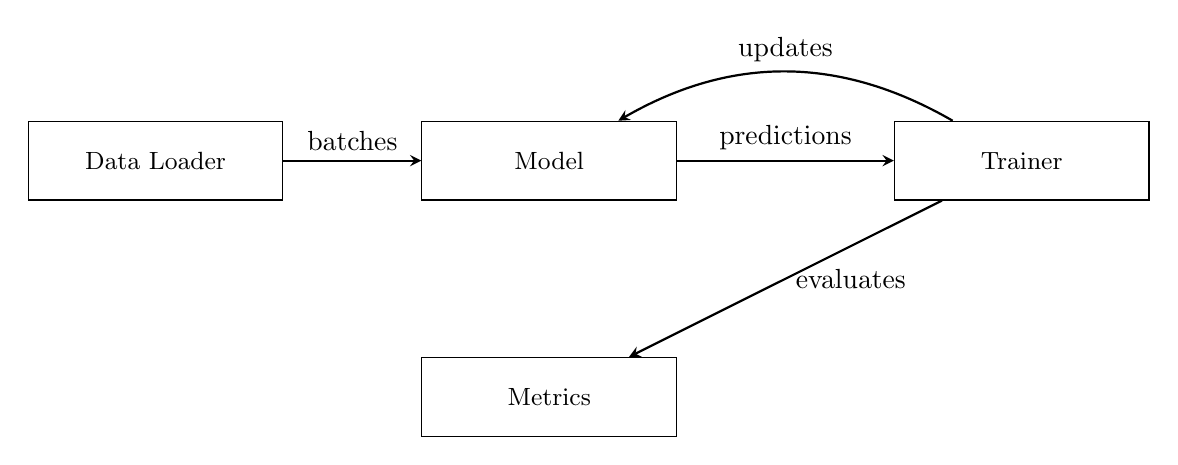
\begin{tikzpicture}[node distance=2cm, auto,
            block/.style={rectangle, draw, text width=3cm, text centered, minimum height=1cm, font=\small},
            arrow/.style={->, >=stealth, thick}]

        \node[block] (loader) {Data Loader};
        \node[block, right of=loader, node distance=5cm] (model) {Model};
        \node[block, right of=model, node distance=6cm] (trainer) {Trainer};
        \node[block, below of=model, node distance=3cm] (metrics) {Metrics};

        \draw[arrow] (loader) -- node[above] {batches} (model);
        \draw[arrow] (model) -- node[above] {predictions} (trainer);
        \draw[arrow] (trainer) -- node[right] {evaluates} (metrics);
        \draw[arrow] (trainer) to[bend right=30] node[above] {updates} (model);
    \end{tikzpicture}
    \caption{Component interaction during training.}
    \label{fig:component_interaction}
\end{figure}

The data loader provides batched hyperspectral images to the model.
The trainer orchestrates the training loop: it calls the model's forward pass, computes the loss, performs backpropagation, and updates model weights.
Metrics are computed periodically (typically each epoch) on the validation set to monitor training progress without affecting the optimization.

This separation ensures that each component has a single responsibility:
\begin{itemize}
    \item \textbf{Loader}: I/O and batching
    \item \textbf{Model}: Forward computation
    \item \textbf{Trainer}: Optimization loop and checkpointing
    \item \textbf{Metrics}: Evaluation
\end{itemize}

\subsection{Metrics}
All metrics are implemented in \mintinline{Python}|Code/metrics/metrics.py|.
\subsubsection{CompressionMetrics class}
The CompressionMetrics class provides static methods for evaluating hyperspectral image compression quality.
The metrics fall into two categories:
\begin{itemize}
    \item {\bf Spatial quality metrics}: MSE, RMSE, PSNR, SNR, and SSIM measure reconstruction fidelity in the spatial domain.
    \item {\bf Spectral quality metrics}: Spectral Angle Mapper (SAM) measures preservation of spectral signatures, which is critical for hyperspectral applications where spectral fidelity matters more than spatial appearance.
\end{itemize}
Additional methods compute compression-specific metrics: compression ratio (CR), bits per pixel (bpp), and bits per pixel per band (bpppb).
\subsubsection{Metrics and loss layer classes}
In addition to the static methods, the \mintinline{Python}|Code/metrics/metrics.py| file also contains several classes that implement the metrics as Keras layers.
These were created to speed up the computation of metrics during model training and evaluation.
The classes are: \mintinline{python}|MeanSquaredError|, \mintinline{python}|PeakSignalToNoiseRatio|, \mintinline{python}|StructualSimilarity| and \\ \mintinline{python}|SpectralAngle|.
Each of these classes inherits from the \mintinline{python}|tf.keras.layers.Layer| class and implements the respective metric in the \mintinline{python}|call| method.
\subsection{Data Loader}
The data loader is implemented in \mintinline{Python}|Code/TFDataloader/TFdataloader.py| as the TFHySpecNetLoader class.
This class utilizes TensorFlow's \mintinline{Python}|tf.data| pipeline to efficiently load and preprocess the HySpecNet-11k dataset.

The loader assumes hyperspectral data stored as NumPy files (\mintinline{bash}|.npy|) with band-major ordering, following the preprocessed format described in the external specification.
Dataset splits are defined by CSV files containing patch identifiers for training, validation, and test sets.

To avoid I/O bottlenecks during training, the loader uses parallel mapping \\(\mintinline{python}|tf.data.AUTOTUNE|) to load multiple files concurrently and prefetching to overlap data loading with model computation.
This design ensures that GPU utilization remains high even when loading large hyperspectral images from disk.

\subsection{Configuration and extensibility}
Model hyperparameters are stored in JSON configuration files (e.g.,\\ \mintinline{bash}|config/lineRWKV_config.json|) rather than being hardcoded.
This separation of configuration from code enables:
\begin{itemize}
    \item Running experiments with different hyperparameters without code changes
    \item Reproducing experiments by storing configuration alongside model weights
    \item Version control of experimental settings
\end{itemize}

To add a new compression model, the following components need to be implemented:
\begin{enumerate}
    \item A model class inheriting from \mintinline{Python}|tf.keras.Model| with \mintinline{Python}|encode| and \mintinline{Python}|decode| methods
    \item A trainer class following the pattern established by LineRWKVTrainer or RCGDNAETrainer
    \item A configuration file specifying model hyperparameters
\end{enumerate}

The existing metrics and data loader can be reused without modification, as they are model-agnostic.
